\documentclass[11pt,a4paper,]{article}
\usepackage{lmodern}

\usepackage{amssymb,amsmath}
\usepackage{ifxetex,ifluatex}
\usepackage{fixltx2e} % provides \textsubscript
\ifnum 0\ifxetex 1\fi\ifluatex 1\fi=0 % if pdftex
  \usepackage[T1]{fontenc}
  \usepackage[utf8]{inputenc}
\else % if luatex or xelatex
  \usepackage{unicode-math}
  \defaultfontfeatures{Ligatures=TeX,Scale=MatchLowercase}
\fi
% use upquote if available, for straight quotes in verbatim environments
\IfFileExists{upquote.sty}{\usepackage{upquote}}{}
% use microtype if available
\IfFileExists{microtype.sty}{%
\usepackage[]{microtype}
\UseMicrotypeSet[protrusion]{basicmath} % disable protrusion for tt fonts
}{}
\PassOptionsToPackage{hyphens}{url} % url is loaded by hyperref
\usepackage[unicode=true]{hyperref}
\hypersetup{
            pdftitle={Fast forecast reconciliation using linear models},
            pdfkeywords={hierarchical forecasting, grouped forecasting, reconciling forecast,
linear regression},
            pdfborder={0 0 0},
            breaklinks=true}
\urlstyle{same}  % don't use monospace font for urls
\usepackage{geometry}
\geometry{left=2.5cm,right=2.5cm,top=2.5cm,bottom=2.5cm}
\usepackage[style=authoryear-comp,]{biblatex}
\addbibresource{references.bib}
\usepackage{longtable,booktabs}
% Fix footnotes in tables (requires footnote package)
\IfFileExists{footnote.sty}{\usepackage{footnote}\makesavenoteenv{long table}}{}
\IfFileExists{parskip.sty}{%
\usepackage{parskip}
}{% else
\setlength{\parindent}{0pt}
\setlength{\parskip}{6pt plus 2pt minus 1pt}
}
\setlength{\emergencystretch}{3em}  % prevent overfull lines
\providecommand{\tightlist}{%
  \setlength{\itemsep}{0pt}\setlength{\parskip}{0pt}}
\setcounter{secnumdepth}{5}

% set default figure placement to htbp
\makeatletter
\def\fps@figure{htbp}
\makeatother


\title{Fast forecast reconciliation using linear models}

%% MONASH STUFF

%% CAPTIONS
\RequirePackage{caption}
\DeclareCaptionStyle{italic}[justification=centering]
 {labelfont={bf},textfont={it},labelsep=colon}
\captionsetup[figure]{style=italic,format=hang,singlelinecheck=true}
\captionsetup[table]{style=italic,format=hang,singlelinecheck=true}

%% FONT
\RequirePackage{bera}
\RequirePackage{mathpazo}

%% HEADERS AND FOOTERS
\RequirePackage{fancyhdr}
\pagestyle{fancy}
\rfoot{\Large\sffamily\raisebox{-0.1cm}{\textbf{\thepage}}}
\makeatletter
\lhead{\textsf{\expandafter{\@title}}}
\makeatother
\rhead{}
\cfoot{}
\setlength{\headheight}{15pt}
\renewcommand{\headrulewidth}{0.4pt}
\renewcommand{\footrulewidth}{0.4pt}
\fancypagestyle{plain}{%
\fancyhf{} % clear all header and footer fields
\fancyfoot[C]{\sffamily\thepage} % except the center
\renewcommand{\headrulewidth}{0pt}
\renewcommand{\footrulewidth}{0pt}}

%% MATHS
\RequirePackage{bm,amsmath}
\allowdisplaybreaks

%% GRAPHICS
\RequirePackage{graphicx}
\setcounter{topnumber}{2}
\setcounter{bottomnumber}{2}
\setcounter{totalnumber}{4}
\renewcommand{\topfraction}{0.85}
\renewcommand{\bottomfraction}{0.85}
\renewcommand{\textfraction}{0.15}
\renewcommand{\floatpagefraction}{0.8}

%\RequirePackage[section]{placeins}

%% SECTION TITLES
\RequirePackage[compact,sf,bf]{titlesec}
\titleformat{\section}[block]
  {\fontsize{15}{17}\bfseries\sffamily}
  {\thesection}
  {0.4em}{}
\titleformat{\subsection}[block]
  {\fontsize{12}{14}\bfseries\sffamily}
  {\thesubsection}
  {0.4em}{}
\titlespacing{\section}{0pt}{*5}{*1}
\titlespacing{\section}{0pt}{*2}{*0.2}


%% TITLE PAGE
\def\Date{\number\day}
\def\Month{\ifcase\month\or
 January\or February\or March\or April\or May\or June\or
 July\or August\or September\or October\or November\or December\fi}
\def\Year{\number\year}

\makeatletter
\def\wp#1{\gdef\@wp{#1}}\def\@wp{??/??}
\def\jel#1{\gdef\@jel{#1}}\def\@jel{??}
\def\showjel{{\large\textsf{\textbf{JEL classification:}}~\@jel}}
\def\nojel{\def\showjel{}}
\def\addresses#1{\gdef\@addresses{#1}}\def\@addresses{??}
\def\cover{{\sffamily\setcounter{page}{0}
        \thispagestyle{empty}%
        \vspace*{-2cm}
        \centerline{\raisebox{-1.8cm}{
\includegraphics[width=5cm]{MBSportrait}}\hspace*{9cm} ISSN 1440-771X}\vspace{0.99cm}
        \begin{center}\Large
        Department of Econometrics and Business Statistics\\[.5cm]
        \scriptsize http://business.monash.edu/econometrics-and-business-statistics/research/publications
        \end{center}\vspace{2cm}
        \begin{center}
        \fbox{\parbox{14cm}{\begin{onehalfspace}\centering\Huge\vspace*{0.3cm}
                \textsf{\textbf{\expandafter{\@title}}}\vspace{1cm}\par
                \LARGE\@author\end{onehalfspace}
        }}
        \end{center}
        \vfill
                \begin{center}\Large
                \Month~\Year\\[1cm]
                Working Paper \@wp
        \end{center}}}
\def\pageone{{\sffamily\setstretch{1}%
        \thispagestyle{empty}%
        \vbox to \textheight{%
        \raggedright\baselineskip=1.2cm
     {\fontsize{24.88}{30}\sffamily\textbf{\expandafter{\@title}}}
        \vspace{2cm}\par
        \hspace{1cm}\parbox{14cm}{\sffamily\large\@addresses}\vspace{1cm}\vfill
        \hspace{1cm}{\large\Date~\Month~\Year}\\[1cm]
        \hspace{1cm}\showjel\vss}}}
\def\blindtitle{{\sffamily
     \thispagestyle{plain}\raggedright\baselineskip=1.2cm
     {\fontsize{24.88}{30}\sffamily\textbf{\expandafter{\@title}}}\vspace{1cm}\par
        }}
\def\titlepage{{\cover\newpage\pageone\newpage\blindtitle}}

\def\blind{\def\titlepage{{\blindtitle}}\let\maketitle\blindtitle}
\def\titlepageonly{\def\titlepage{{\pageone\end{document}}}}
\def\nocover{\def\titlepage{{\pageone\newpage\blindtitle}}\let\maketitle\titlepage}
\let\maketitle\titlepage
\makeatother

%% SPACING
\RequirePackage{setspace}
\spacing{1.5}

%% LINE AND PAGE BREAKING
\sloppy
\clubpenalty = 10000
\widowpenalty = 10000
\brokenpenalty = 10000
\RequirePackage{microtype}

%% PARAGRAPH BREAKS
\setlength{\parskip}{1.4ex}
\setlength{\parindent}{0em}

%% HYPERLINKS
\RequirePackage{xcolor} % Needed for links
\definecolor{darkblue}{rgb}{0,0,.6}
\RequirePackage{url}

\makeatletter
\@ifpackageloaded{hyperref}{}{\RequirePackage{hyperref}}
\makeatother
\hypersetup{
     citecolor=0 0 0,
     breaklinks=true,
     bookmarksopen=true,
     bookmarksnumbered=true,
     linkcolor=darkblue,
     urlcolor=blue,
     citecolor=darkblue,
     colorlinks=true}

%% KEYWORDS
\newenvironment{keywords}{\par\vspace{0.5cm}\noindent{\sffamily\textbf{Keywords:}}}{\vspace{0.25cm}\par\hrule\vspace{0.5cm}\par}

%% ABSTRACT
\renewenvironment{abstract}{\begin{minipage}{\textwidth}\parskip=1.4ex\noindent
\hrule\vspace{0.1cm}\par{\sffamily\textbf{\abstractname}}\newline}
  {\end{minipage}}


\usepackage[T1]{fontenc}
\usepackage[utf8]{inputenc}

\usepackage[showonlyrefs]{mathtools}
\usepackage[no-weekday]{eukdate}

%% BIBLIOGRAPHY

\makeatletter
\@ifpackageloaded{biblatex}{}{\usepackage[style=authoryear-comp, backend=biber, natbib=true]{biblatex}}
\makeatother
\ExecuteBibliographyOptions{bibencoding=utf8,minnames=1,maxnames=3, maxbibnames=99,dashed=false,terseinits=true,giveninits=true,uniquename=false,uniquelist=false,doi=false, isbn=false,url=true,sortcites=false}

\DeclareFieldFormat{url}{\texttt{\url{#1}}}
\DeclareFieldFormat[article]{pages}{#1}
\DeclareFieldFormat[inproceedings]{pages}{\lowercase{pp.}#1}
\DeclareFieldFormat[incollection]{pages}{\lowercase{pp.}#1}
\DeclareFieldFormat[article]{volume}{\mkbibbold{#1}}
\DeclareFieldFormat[article]{number}{\mkbibparens{#1}}
\DeclareFieldFormat[article]{title}{\MakeCapital{#1}}
\DeclareFieldFormat[article]{url}{}
%\DeclareFieldFormat[book]{url}{}
%\DeclareFieldFormat[inbook]{url}{}
%\DeclareFieldFormat[incollection]{url}{}
%\DeclareFieldFormat[inproceedings]{url}{}
\DeclareFieldFormat[inproceedings]{title}{#1}
\DeclareFieldFormat{shorthandwidth}{#1}
%\DeclareFieldFormat{extrayear}{}
% No dot before number of articles
\usepackage{xpatch}
\xpatchbibmacro{volume+number+eid}{\setunit*{\adddot}}{}{}{}
% Remove In: for an article.
\renewbibmacro{in:}{%
  \ifentrytype{article}{}{%
  \printtext{\bibstring{in}\intitlepunct}}}

\AtEveryBibitem{\clearfield{month}}
\AtEveryCitekey{\clearfield{month}}

\makeatletter
\DeclareDelimFormat[cbx@textcite]{nameyeardelim}{\addspace}
\makeatother
\renewcommand*{\finalnamedelim}{%
  %\ifnumgreater{\value{liststop}}{2}{\finalandcomma}{}% there really should be no funny Oxford comma business here
  \addspace\&\space}


\wp{no/yr}
\jel{C10,C14,C22}

\nocover

\author{Mahsa~Ashouri, Rob J~Hyndman, Galit~Shmueli}
\addresses{\textbf{Mahsa Ashouri}\newline
Institute of Service Science, National Tsing Hua University, Taiwan
\newline{Email: \href{mailto:mahsa.ashouri@iss.nthu.edu.tw}{\nolinkurl{mahsa.ashouri@iss.nthu.edu.tw}}}\newline Corresponding author\\[1cm]
\textbf{Rob J Hyndman}\newline
Monash University, Clayton VIC 3800, Australia
\newline{Email: \href{mailto:rob.hyndman@monash.edu}{\nolinkurl{rob.hyndman@monash.edu}}}\\[1cm]
\textbf{Galit Shmueli}\newline
Institute of Service Science, National Tsing Hua University, Taiwan
\newline{Email: \href{mailto:galit.shmueli@iss.nthu.edu.tw}{\nolinkurl{galit.shmueli@iss.nthu.edu.tw}}}\\[1cm]
}

\date{\sf\Date~\Month~\Year}
\makeatletter
 \lfoot{\sf Ashouri, Hyndman, Shmueli: \@date}
\makeatother

%% Any special functions or other packages can be loaded here.


 \usepackage{booktabs}
 \usepackage{float}
\usepackage{longtable}
\usepackage{cases}
\usepackage{array}
%\usepackage[backend=biber]{biblatex}
%\usepackage[backend=biber, bibencoding=utf8, style=authoryear, citestyle=authoryear]{biblatex}


\begin{document}
\maketitle
\begin{abstract}
Available package for forecasting hierarchical and grouped time series
is \textbf{hts}. This package uses Exponential Smoothing (ets) and
Autoregressive Integrated Moving Average (ARIMA) for computing base
forecasts which can be computationally chalanging for large collection
of time series. In this paper we propose a linear approach which can
adjust computation time with good accuracy level. We illustrate our
approach using two datasets, Australian domestic tourism and Wikipedia
pageview datasets. In these two datasets we compare our approach with
ets and ARIMA. We show that our approach is much faster and can compete
these two methods in case of forecasting accuracy level. We also show
the effect of reconceliation step on the accuracy level in all the three
methods.
\end{abstract}
\begin{keywords}
hierarchical forecasting, grouped forecasting, reconciling forecast,
linear regression
\end{keywords}

\section{Introduction}\label{introduction}

\subsection{Hierarchical and grouped time
series}\label{hierarchical-and-grouped-time-series}

One of the consequences of increasing internet usage and life digitizing
is increasing the amount of collected time series data. As an example we
can refer to the Internet of Things (IoT) which produces huge amount of
series in short period of time. Forecasting large collection of time
series is always computationally heavy and challenging. In some cases
these time series can be structured and disaggregated based on
hierarchies or groups such as geographical location and gender. One
example for hierarchical time series can be the amount of sales in
restaurant chains which can be disaggregated into different branches and
then foods or drinks. One visualizing example of these time series
structure is shown in Figure \ref{fig:hierarchicalexample}. In this
example the hierarchy includes three levels. Top level, level 0, is the
total series which is the aggregation of all the bottom level series,
the middle level, level 1, series are aggregation of their own bottom
level series for instance series A is the aggregation of AA and AB and
finally the bottom level , level 2, series which includes the most
disaggregated series.

Grouped time series are more complicated aggregation structure in
compare with hierarchical time series. They can be defined as
hierarchical time series without unique hierarchy structure
\autocite{hyndman2015hts}. All the computations, notations and
approaches can be used for them as well.

\begin{figure}

{\centering 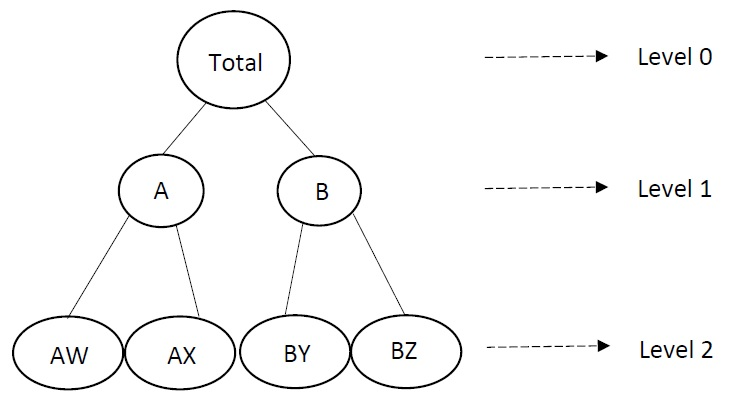
\includegraphics[width=280px,height=180px]{Paper-Figures/hierarchical_example} 

}

\caption{An example of two level hierarchy structure}\label{fig:hierarchicalexample}
\end{figure}

Back to the notations used by \textcite{hyndman2016fast}, we call the
total series for \(t\)th observation by \(y_t\) and the \(t\)th
observation at the node \(Z\) by \(y_{Z,t}\). For generating different
levels series from bottom level series, there is a matrix which is
called \(n\times n_k\) `summing matrix' denoted by \(S\), which \(n\) is
the number of all the nodes and \(n_k\) is the number of bottom level
nodes. This summing matrix can be partitioned based on different level
of hierarchy. Using `summing matrix', the notation for generation
hierarchy structure is \(\mathbf{y_t}=\mathbf{Sb_t}\). Where
\(\mathbf{y_t}\) is a vector of all the level nodes or all the
observations and \(\mathbf{b_t}\) is the vector of all the bottom level
nodes of hierarchy at time \(t\). For the example shown in Figure
\ref{fig:hierarchicalexample} the hierarchy equation involving
\(S_{7\times 4}\) matrix can be written as follows:

\[
\left(\begin{array}{c} 
y_{t}\\y_{A,t}\\y_{B,t}\\y_{AA,t}\\y_{AB,t}\\y_{BA,t}\\y_{BB,t}\\
\end{array}\right)
=\left(\begin{array}{cccc} 
1&1&1&1\\1&1&0&0\\0&0&1&1\\1&0&0&0\\0&1&0&0\\0&0&1&0\\0&0&0&1\\
\end{array}\right)
\left(\begin{array}{c} 
y_{AA,t}\\y_{AB,t}\\y_{BA,t}\\y_{BB,t}\\
\end{array}\right)
\]

\subsection{Forecasting hierarchical time
series}\label{forecasting-hierarchical-time-series}

In hierarchical time series forecasting all the individual series can
affect the accuracy level, since the most disaggregated or bottom level
series are highly noisy and then their forecasting results are not that
accurate and the most aggregated or total series, is smoother and less
noisy though forecasting them is easier
\autocite{fliedner2001hierarchical}. On the other hand, we are ignoring
hierarchy or grouping structure and there is no level structure in the
forecasted series if we just forecast each series individually
\autocite{hyndman2016fast}. Also, forecasting the most disaggregated
level series and computing other level series by summing forecasts can
result poor forecasts at higher level.

In literature there are some methods which consider hierarchy structure
information in forecasting time series including top-down
\autocite{gross1990disaggregation}, bottom-up
\autocite{kahn1998revisiting}, middle-out and optimal combination
\autocite{hyndman2011optima} approaches. In top-down approach we first
forecast the total series and then disaggregate the forecast to bottom
level series based on a set of historical and forecasted proportions (
details about proportions in \textcite{athanasopoulos2009hierarchical}).
In bottom-up approach the forecasts in each level of hierarchy can be
computed using aggregating the bottom level series forecast. In
middle-out approach, the process can be started from one of the middle
levels and other forecasted can be computed using aggregation for upper
levels and disaggregation for lower levels. Finally optimal combination
uses all the base forecasts, forecasts for all the series in the whole
hierarchy structure, then applies some regression models to reconcile
those base forecasts. The advantage of the latest methods in compare
with other methods is that it considers the interactions and correlation
among the series in all the levels of hierarchy. The optimal combination
method is based on the forecasting all the series is all the level of
hierarchy, which is called `base forecasts', and then using a kind of
regression model to combine and reconcile those forecast optimally. This
method also provides forecast uncertainty and flexible for ad hoc
adjustment.

In this method, base forecasts can be computed using the following
linear model:

\begin{equation}\label{eq:baseforecasts}
   \mathbf{\hat{y}_h} = \mathbf{S}\boldsymbol{\beta_h}+\epsilon_h
\end{equation}

where \(\mathbf{\hat{y}_h}\) represents a vector of \(h\)-step-ahead
base forecasts for all levels of the hierarchy, \(\boldsymbol{\beta_h}\)
is the unknown conditional mean of the bottom level series and
\(\epsilon_h\) is the aggregation error which has mean equal to zero and
variance equal to \(\sum_h\) \autocite{hyndman2016fast}. Using the
Equation \eqref{eq:baseforecasts}, by estimating \(\boldsymbol{\beta_h}\)
forecasts in all levels of hierarchy can be computed. Since estimating
\(\boldsymbol{\beta_h}\) using Generalized Least Square (GLS) need
knowledge about \(\sum_h\), Ordinary Least Square (OLS) can be used over
it for this estimation and then a vector of reconciled forecast can be
calculated using Equation \eqref{eq:reconciledforecasts}.

\begin{equation}\label{eq:reconciledforecasts}
   \mathbf{\tilde{y}_{h}}=\mathbf{S(S'S)^{-1}S'}\mathbf{\hat{y}_h}
\end{equation}

\subsection{Challenges and
motivations}\label{challenges-and-motivations}

In 2015 \textcite{hyndman2015hts} implemented a package called
\textbf{hts} in R (\textcite{team2013r}) for forecasting hierarchical
time series including all the mentioned approaches in the last section.
In this package two functions, \emph{hts} and \emph{gts}, produce
hierarchical time series respectively. Inputs for these functions
include base forecasts and hierarchy and group structure. Here base
forecasts are forecasts in all levels of hierarchy using only the
history of each series and ignoring hierarchy or group structure. In
optimal combination method, there are two steps to determine the
reconciled forecasts first computing base forecasts and second
reconciling those forecasts. Currently options for computing the base
forecasts are Random Walk (rw), Exponential Smoothing (ets),
Autoregressive Integrated Moving Average (ARIMA).

When we encounter large collection of time series computing base
forecasts using ets or ARIMA can be computationally expensive. In this
research we are proposing a new linear function to calculate the base
forecasts fast with acceptable accuracy level.

\section{Proposed approach}\label{proposed-approach}

Our proposed approach is based on using linear regression models for
computing base forecasts using different set of predictors. Following
the above notations, lets use \(\mathbf{y_t}\) for the vector of
response variables in training set for for all the level of hierarchy
and for \(h\)-step-ahead base forecasts and reconciled vector we use
\(\mathbf{\widehat{y}_{h}}\) and \(\mathbf{\tilde{y}_{h}}\). We also use
\(X\) as a matrix of predictors and \(\mathbf{X_t}\) and
\(\mathbf{X_h}\) for the matrix of predictor in training and test set.

We present our linear model in Equation \eqref{eq:linearmodel}, where
\(\boldsymbol{\alpha_h}\) represents the vector of linear model
coefficients and \(\delta\) is the error term with mean zero and
constant variance.

\begin{equation}\label{eq:linearmodel}
   \mathbf{y_t} = \mathbf{X_t} \boldsymbol{\alpha_h}+\delta 
\end{equation}

Then we can estimate the coefficients in Equation \eqref{eq:linearmodel}
as follows:

\begin{equation}\label{eq:linearcoefficients}
   \boldsymbol{\hat{\alpha}_h} = \mathbf{(X'X)^{-1}X'}\mathbf{y_t}
\end{equation}

Finally using Equation \eqref{eq:reconciledforecasts} and
\eqref{eq:linearcoefficients}, reconciled forecast coefficients can be
computed by Equation \eqref{eq:reconciledcoefficients}.

\begin{equation}\label{eq:reconciledcoefficients}
   \boldsymbol{\tilde{\beta}_h} = \mathbf{(S'S)^{-1}S'}\mathbf{y_t}\mathbf{X(X'X)^{-1}}\mathbf{X_h}
\end{equation}

As an example for the \(\mathbf{X}\) matrix in Equation
\eqref{eq:linearmodel}, we can refer the set of predictors proposed in
\textcite{ashouri2018} In this paper they suggested using linear trend,
dummy seasonality and time series lags as a set of predictors in linear
model to forecast large collection of time series. Equation
\eqref{eq:linearmodelexample} shows this linear equation where \(y_t\)
represent series at time \(t\), and \(Season_j\) is a dummy variable
taking value 1 if time \(j\) is in season \(j\). Further, \(y_{t-j}\) is
the \(j\)th lagged value for \(y_t\). For instance, if we have daily
data with day of week seasonality, \(j\) would be 7 (7 seasonal dummies
and 7 time series lags).

\begin{equation}\label{eq:linearmodelexample}
   y_t = \alpha_0 + \alpha_1 t + \beta_1 Season_{1t} + \beta_2 Season_{2t} + \cdots + \beta_m Season_{mt} + \gamma_1 y_{t-1} + \gamma_2 y_{t-2} + \cdots + \gamma_m y_{t-m} 
\end{equation}

\section{Applications}\label{applications}

In this section we are illustrating our approach and its results using
two examples, Australian domestic tourism and Wikipedia pageview
datasets. We are comparing the forecasting accuracy levels among ets,
ARIMA and the proposed model, OLS, with and without reconciliation step
on forecasting. For comparing these methods we use average of Root Mean
Square Error (RMSE) and error plot along with the raw forecasted errors.
Since we are using time series lags in our approach (OLS), we can not
forecast multiple step ahead then we apply two methods for forecasting
\(h\)-step-ahead forecast, which \(h\) is the the number of desired
forecast. In first one, for forecasting each point of the forecasting
interval we use 1-step-ahead forecast and for forecasting the following
point we replace the last point with the actual value. In our
applications, we call this approach 1-step-ahead. In the second method,
we forecast each point of forecasting interval we use 1-step-ahead
forecast and for forecasting the following point we use that last
forecasted point. In our applications, we call this approach
\(h\)-step-ahead forecast. We also show the computation challenges in
all the methods.

\subsection{Australian domestic tourism
dataset}\label{australian-domestic-tourism-dataset}

This dataset is 19 years (1998-2017) quarterly and measured by
Australians visitor nights spend away from home collected each month
\autocite{wickramasuriya2018optimal}. In total this dataset includes 304
time series with length 228 each. The hierarchy and grouping structure
for this dataset is made using geographical and purpose information. In
this dataset we have three levels geographical division for Australia.
In the first level Australia was divided into seven `State' including
New South Wales (NSW), Victoria (VIC), Queensland (QLD), South Australia
(SA), Western Australia (WA), Tasmania (TAS) and Northern Territory
(NT). In the second and third levels its divided into 27 `Zone' and 76
`Region' (details about Australia geographical division in Table
\ref{tab:Australiageographicaldivision}). Also for `Purpose' we provided
with four groups: Holiday (Hol), Visiting (Vis), Business (Bis) and
Others (Oth). Based on geographical hierarchy and purpose grouping, we
end up with 8 levels of hierarchy with 555 series in total (check Table
\ref{tab:Australiageographicalpurposedivision} from
\autocite{wickramasuriya2018optimal}). The hierarchy structure which is
used in this example includes these levels: level0 = Total series,
level1 = State, level 2 = Zone, level3 = Region, level4 = Purpose,
level5 = State \(\times\) Purpose, level6 = Zone \(\times\) Purpose and
level7 = bottom level series. We report the forecast results for all
these hierarchy levels in this example.

In our predictor matrix, we apply linear trend, since this dataset
collected every month 12 dummy seasonal variables and since it is
quarterly datast 4 time series lags.

\begin{table}[t]

\caption{\label{tab:Australiageographicaldivision}Australia geographical hierarchy structure}
\centering
\fontsize{9}{11}\selectfont
\begin{tabular}{crccrc}
\toprule
Series & Name & Lable & Series & Name & Lable\\
\midrule
Total &  &  & Region &  & \\
1 & Australia & Total & 55 & Lakes & BCA\\
State &  &  & 56 & Gippsland & BCB\\
2 & NSW & A & 57 & Phillip Island & BCC\\
3 & VIC & B & 58 & General Murray & BDA\\
4 & QLD & C & 59 & Goulburn & BDB\\
5 & SA & D & 60 & High Country & BDC\\
6 & WA & E & 61 & Merbourne East & BDD\\
7 & TAS & F & 62 & Upper Yarra & BDE\\
8 & NT & G & 63 & Murray East & BDF\\
Zone &  &  & 64 & Wimmera+Mallee & BEA\\
9 & Metro NSW & AA & 65 & Western Grampians & BEB\\
10 & Nth Coast NSW & AB & 66 & Bendigo Loddon & BEC\\
11 & Sth Coast NSW & AC & 67 & Macedon & BED\\
12 & Sth NSW & AD & 68 & Spa Country & BEE\\
13 & Nth NSW & AE & 69 & Ballarat & BEF\\
14 & ACT & AF & 70 & Central Highlands & BEG\\
15 & Metro VIC & BA & 71 & Gold Coast & CAA\\
16 & West Coast VIC & BB & 72 & Brisbane & CAB\\
17 & East Coast VIC & BC & 73 & Sunshine Coast & CAC\\
18 & Nth East VIC & BD & 74 & Central Queensland & CBA\\
19 & Nth West VIC & BE & 75 & Bundaberg & CBB\\
20 & Metro QLD & CA & 76 & Fraser Coast & CBC\\
21 & Central Coast QLD & CB & 77 & Mackay & CBD\\
22 & Nth Coast QLD & CC & 78 & Whitsundays & CCA\\
23 & Inland QLD & CD & 79 & Northern & CCB\\
24 & Metro SA & DA & 80 & Tropical North Queensland & CCC\\
25 & Sth Coast SA & DB & 81 & Darling Downs & CDA\\
26 & Inland SA & DC & 82 & Outback & CDB\\
27 & West Coast SA & DD & 83 & Adelaide & DAA\\
28 & West Coast WA & EA & 84 & Barrosa & DAB\\
29 & Nth WA & EB & 85 & Adelaide Hills & DAC\\
30 & Sth WA & EC & 86 & Limestone Coast & DBA\\
31 & Sth TAS & FA & 87 & Fleurieu Peninsula & DBB\\
32 & Nth East TAS & FB & 88 & Kangaroo Island & DBC\\
33 & Nth West TAS & FC & 89 & Murraylands & DCA\\
34 & Nth Coast NT & GA & 90 & Riverland & DCB\\
35 & Central NT & GB & 91 & Clare Valley & DCC\\
Region &  &  & 92 & Flinders Range and Outback & DCD\\
36 & Sydney & AAA & 93 & Eyre Peninsula & DDA\\
37 & Central Coast & AAB & 94 & Yorke Peninsula & DDB\\
38 & Hunter & ABA & 95 & Australia's Coral Coast & EAA\\
39 & North Coast NSW & ABB & 96 & Experience Perth & EAB\\
40 & Northern Rivers Tropical NSW & ABC & 97 & Australia's SouthWest & EAC\\
41 & South Coast & ACA & 98 & Australia's North West & EBA\\
42 & Snowy Mountains & ADA & 99 & Australia's Golden Outback & ECA\\
43 & Capital Country & ADB & 100 & Hobart and the South & FAA\\
44 & The Murray & ADC & 101 & East Coast & FBA\\
45 & Riverina & ADD & 102 & Launceston, Tamar and the North & FBB\\
46 & Central NSW & AEA & 103 & North West & FCA\\
47 & New England North West & AEB & 104 & Wilderness West & FCB\\
48 & Outback NSW & AEC & 105 & Darwin & GAA\\
49 & Blue Mountains & AED & 106 & Kakadu Arnhem & GAB\\
50 & Canberra & AFA & 107 & Katherine Daly & GAC\\
51 & Melbourne & BAA & 108 & Barkly & GBA\\
52 & Peninsula & BAB & 109 & Lasseter & GBB\\
53 & Geelong & BAc & 110 & Alice Springs & GBC\\
54 & Western & BBA & 111 & MacDonnell & GBD\\
\bottomrule
\end{tabular}
\end{table}

\begin{table}[t]

\caption{\label{tab:Australiageographicalpurposedivision}Number of Australian domestic tourism series in each level of hierarchy and group structure}
\centering
\begin{tabular}{>{\centering\arraybackslash}p{3cm}>{\centering\arraybackslash}p{3cm}>{\centering\arraybackslash}p{3cm}>{\centering\arraybackslash}p{3cm}}
\toprule
Geographical devision & \# of series (geographical devision) & \# of series (purpose of travel) & Total\\
\midrule
Australia & 1 & 4 & 5\\
State & 7 & 28 & 35\\
Zone & 27 & 108 & 135\\
Region & 76 & 304 & 380\\
Total & 111 & 444 & 555\\
\bottomrule
\end{tabular}
\end{table}

In Table \ref{tab:Tourismdataresulrolling},
\ref{tab:TourismdataresultRMSE} and
\ref{tab:Tourismdatacomputationtime}, we display the average of RMSE and
computation time for tourism dataset. Methods include ets, ARIMA and our
proposed linear model, OLS. In our OLS model we used linear trend,
seasonal dummies and four lags as our predictors. In Table
\ref{tab:Tourismdataresulrolling} we forecast 24, 1-step-ahead points
and in, all three methods, after each step we replaced the forecasted
point with the actual values to forecast next point. In Table
\ref{tab:TourismdataresultRMSE} we did 24-step-ahead forecast and, in
OLS method, after each step we used that forecasted point to forecast
next point. In these tables we have two parts related to the forecast
with and without reconciliation and also we have the average RMSE for
all the levels of hierarchy, level0=total to level6=bottom level series.

Results in Table \ref{tab:Tourismdataresulrolling} and
\ref{tab:TourismdataresultRMSE} represent the help of reconciliation in
decreasing the average of RMSE in all the three methods, also except for
the total series, reconciliation can help in forecasting all the
hierarchy levels. On the other hand, results show that our proposed OLS
method is competing ets and ARIMA methods which are computationally
heavy for many time series.

\begin{table}[t]

\caption{\label{tab:unnamed-chunk-1}Mean(RMSE) for ets, ARIMA and OLS with and without reconciliation - 1-step-ahead - Tourism dataset}
\centering
\begin{tabular}{ccccccc}
\toprule
\multicolumn{1}{c}{} & \multicolumn{6}{c}{Mean(RMSE)} \\
\cmidrule(l{2pt}r{2pt}){2-7}
\multicolumn{1}{c}{} & \multicolumn{3}{c}{Unreconciled} & \multicolumn{3}{c}{Reconciled} \\
\cmidrule(l{2pt}r{2pt}){2-4} \cmidrule(l{2pt}r{2pt}){5-7}
 & ets & ARIMA & OLS & ets & ARIMA & OLS\\
\midrule
Level 0 & 1516.40 & 1445.49 & 1773.71 & 1533.58 & 1453.44 & 1842.14\\
Level 1 & 511.37 & 493.14 & 550.51 & 495.88 & 457.65 & 523.40\\
Level 2 & 214.81 & 219.01 & 227.56 & 209.16 & 207.52 & 216.33\\
Level 3 & 122.91 & 125.08 & 123.52 & 118.67 & 120.52 & 120.00\\
Level 4 & 675.99 & 709.22 & 721.21 & 668.26 & 679.74 & 718.25\\
Level 5 & 213.06 & 220.08 & 219.17 & 210.64 & 209.39 & 213.54\\
Level 6 & 97.53 & 102.41 & 100.80 & 96.36 & 99.77 & 97.88\\
Level 7 & 56.17 & 58.20 & 57.33 & 55.98 & 57.68 & 56.21\\
\bottomrule
\end{tabular}
\end{table}

\begin{table}[t]

\caption{\label{tab:Tourismdataresulrolling}Mean(RMSE) for ets, ARIMA and OLS with and without reconciliation - 1-step-ahead - Tourism dataset}
\centering
\begin{tabular}{ccccccc}
\toprule
\multicolumn{1}{c}{} & \multicolumn{6}{c}{Mean(RMSE)} \\
\cmidrule(l{2pt}r{2pt}){2-7}
\multicolumn{1}{c}{} & \multicolumn{3}{c}{Unreconciled} & \multicolumn{3}{c}{Reconciled} \\
\cmidrule(l{2pt}r{2pt}){2-4} \cmidrule(l{2pt}r{2pt}){5-7}
 & ets & ARIMA & OLS & ets & ARIMA & OLS\\
\midrule
Level 0 & 1516.40 & 1445.49 & 1773.71 & 1533.58 & 1453.44 & 1842.14\\
Level 1 & 511.37 & 493.14 & 550.51 & 495.88 & 457.65 & 523.40\\
Level 2 & 214.81 & 219.01 & 227.56 & 209.16 & 207.52 & 216.33\\
Level 3 & 122.91 & 125.08 & 123.52 & 118.67 & 120.52 & 120.00\\
Level 4 & 675.99 & 709.22 & 721.21 & 668.26 & 679.74 & 718.25\\
Level 5 & 213.06 & 220.08 & 219.17 & 210.64 & 209.39 & 213.54\\
Level 6 & 97.53 & 102.41 & 100.80 & 96.36 & 99.77 & 97.88\\
Level 7 & 56.17 & 58.20 & 57.33 & 55.98 & 57.68 & 56.21\\
\bottomrule
\end{tabular}
\end{table}

In Figures \ref{fig:errorplotrollingtourism} and
\ref{fig:errorplot24tourism} we display error plots along with the raw
data for forecasted errors of all the series in all the hierarchy levels
for ets, ARIMA and OLS models. In these figures we also compare the
reconcile and unreconcile forecasts. As it is clear from the figures,
error density are more cumulative around zero while we are doing
1-step-ahead forecasting. Also if we compare reconcile forecasts with
unreconcile forecasts, we can conclude that in hierarchy structure
series mostly reconciliation step can improve the forecasts. Finally,
OLS method shows acceptable results in compare with other two methods in
\textbf{hts} package in almost all the levels of hierarchy.

\begin{figure}

{\centering 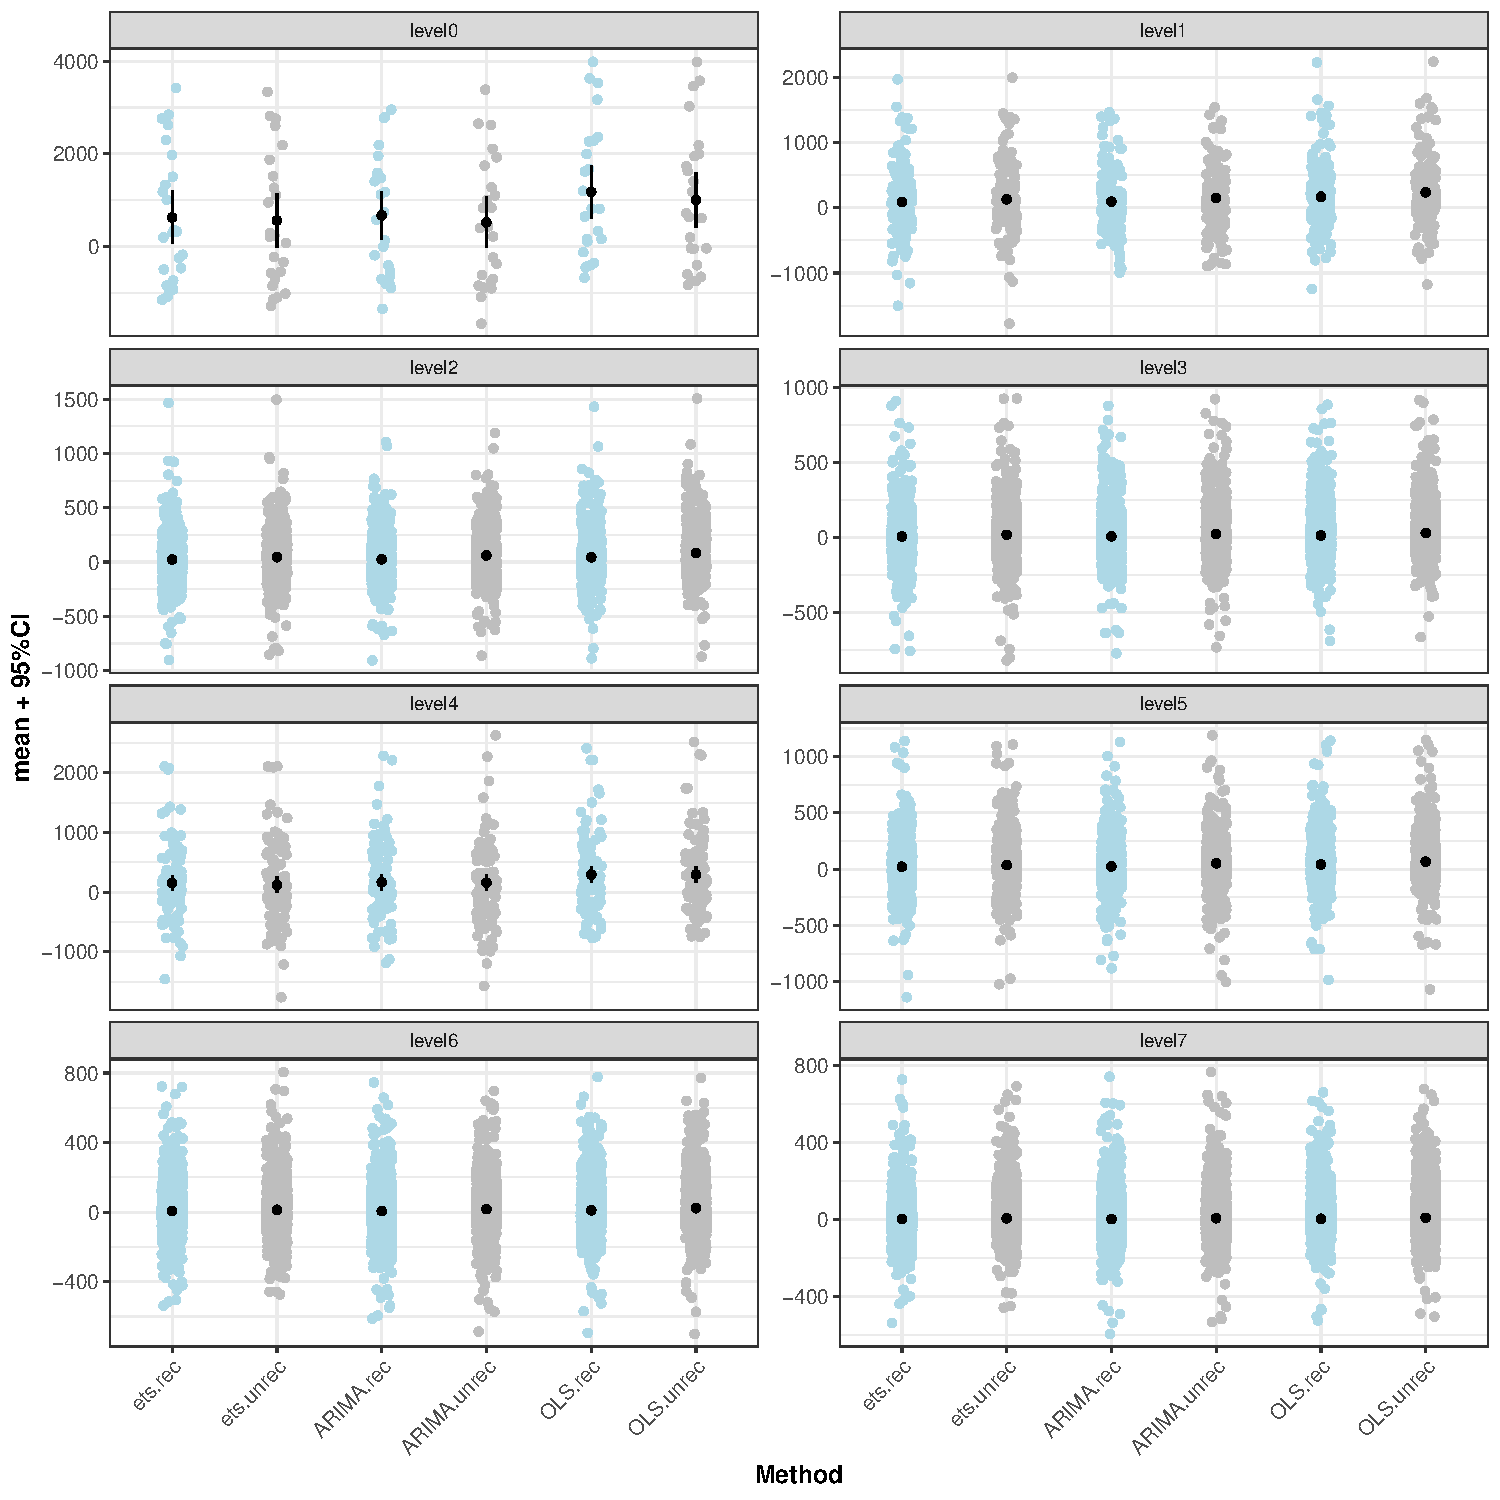
\includegraphics[width=400px,height=300px]{Paper-Figures/results_Tourism/boxplot_raw_data_1_step} 

}

\caption{Mean error plots with raw data -  Reconciled and unreconciled ets, ARIMA and OLS in all the hierarchy level- 1-step-ahead - Tourism dataset}\label{fig:errorplotrollingtourism}
\end{figure}

\begin{table}[t]

\caption{\label{tab:TourismdataresultRMSE}Mean(RMSE) for ets, ARIMA and OLS with and without reconciliation - 24-step-ahead - Tourism dataset}
\centering
\begin{tabular}{ccccccc}
\toprule
\multicolumn{1}{c}{} & \multicolumn{6}{c}{Mean(RMSE)} \\
\cmidrule(l{2pt}r{2pt}){2-7}
\multicolumn{1}{c}{} & \multicolumn{3}{c}{Unreconciled} & \multicolumn{3}{c}{Reconciled} \\
\cmidrule(l{2pt}r{2pt}){2-4} \cmidrule(l{2pt}r{2pt}){5-7}
 & ets & ARIMA & OLS & ets & ARIMA & OLS\\
\midrule
Level 0 & 2238.58 & 3553.99 & 5050.33 & 2250.22 & 3179.39 & 4671.05\\
Level 1 & 593.57 & 570.13 & 900.10 & 553.76 & 626.32 & 902.99\\
Level 2 & 239.52 & 229.64 & 278.84 & 234.21 & 242.46 & 290.95\\
Level 3 & 132.58 & 129.40 & 142.78 & 126.74 & 129.40 & 146.33\\
Level 4 & 766.78 & 824.00 & 1306.97 & 795.48 & 958.24 & 1434.05\\
Level 5 & 226.74 & 241.18 & 298.24 & 222.48 & 236.94 & 308.39\\
Level 6 & 103.02 & 105.38 & 110.91 & 101.95 & 103.93 & 115.36\\
Level 7 & 59.12 & 58.81 & 60.91 & 58.54 & 58.71 & 62.64\\
\bottomrule
\end{tabular}
\end{table}

\begin{figure}

{\centering 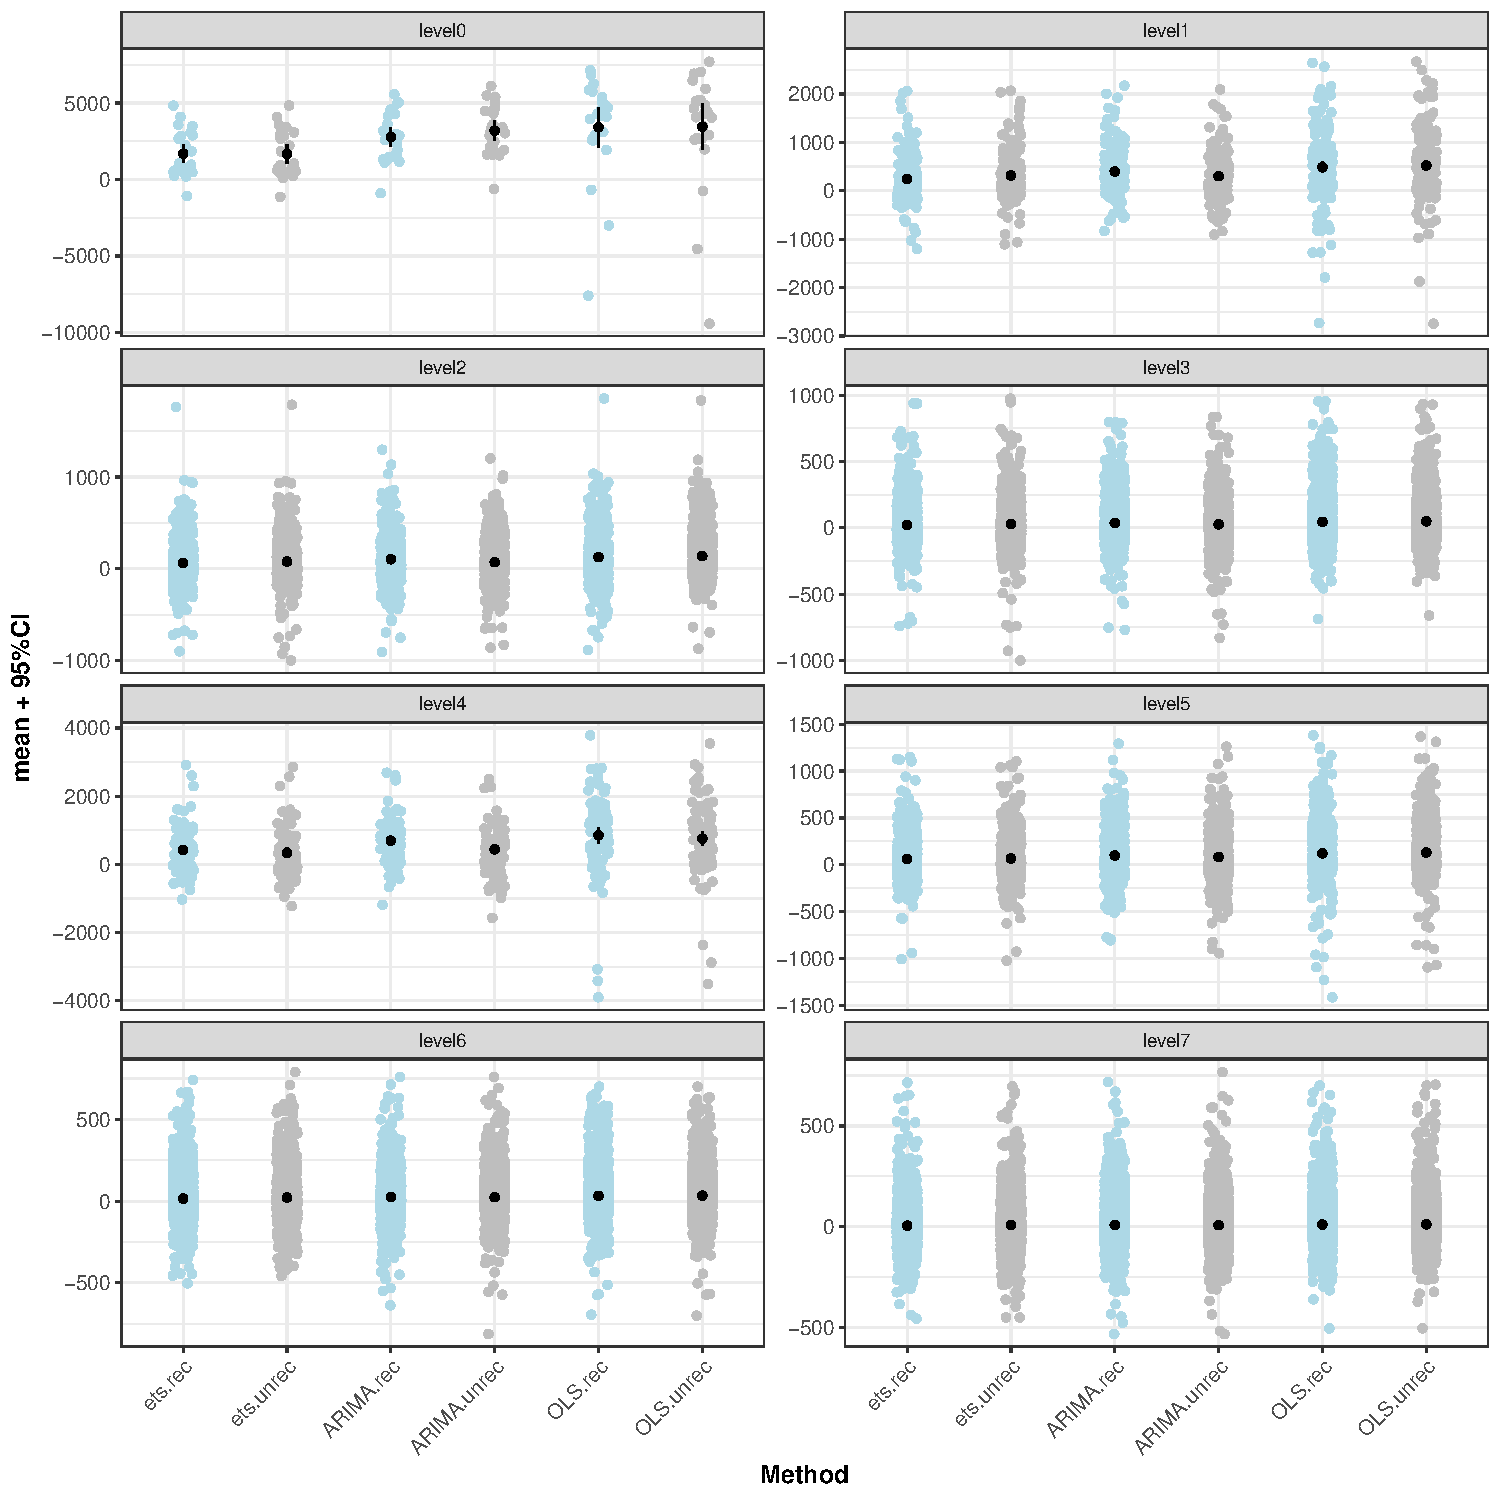
\includegraphics[width=400px,height=300px]{Paper-Figures/results_Tourism/boxplot_raw_data} 

}

\caption{Mean error plots with raw data -  Reconciled and unreconciled ets, ARIMA and OLS in all the hierarchy level- 24-step-ahead - Tourism dataset}\label{fig:errorplot24tourism}
\end{figure}

In Figure \ref{fig:forecstrolling24tourism} we have the 1- and
24-step-ahead forecast results on the test set for one of the bottom
level series, CACBus (Sunshine Coast - Business). In these plots we have
both reconciled (solid lines) and unreconciled (dashed lines) forecast
and we can see that reconceliation step could improve the forecast in
this series. We also can see that OLS forecast result is similar to the
other two methods.

\begin{figure}

{\centering 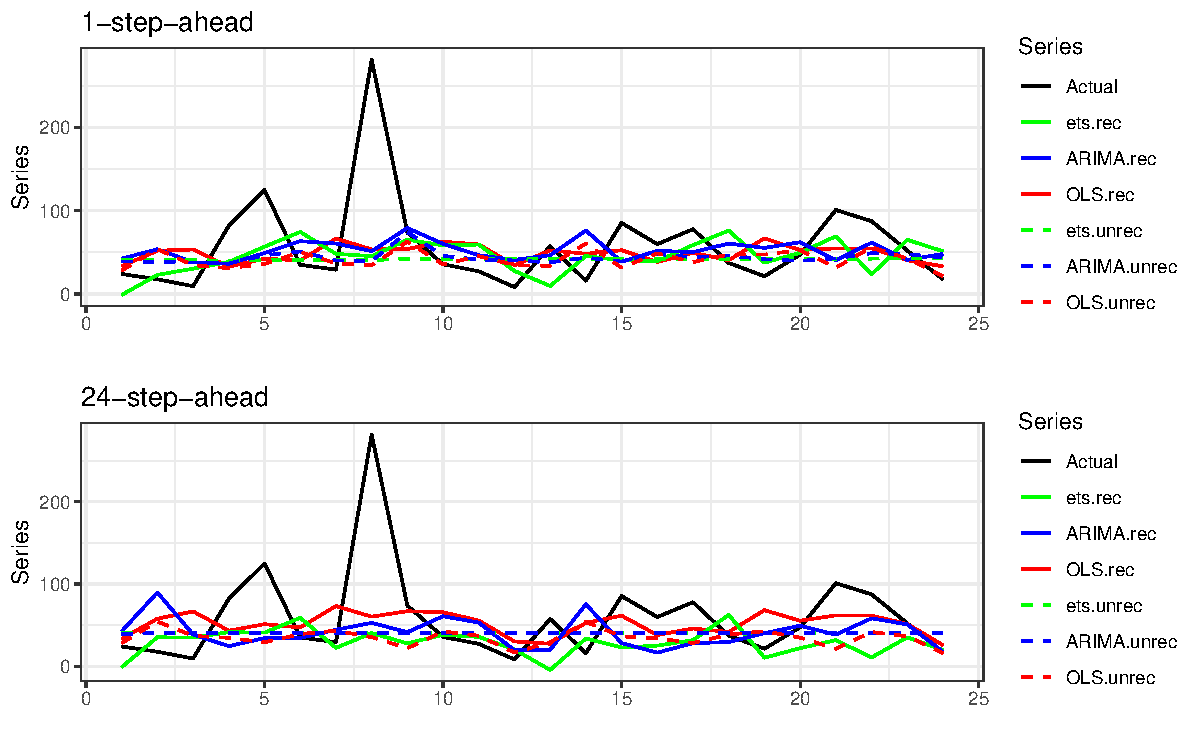
\includegraphics[width=400px,height=300px]{hcf_files/figure-latex/forecstrolling24tourism-1} 

}

\caption{Comparing Actual test set, Reconciled and unreconciled ets, ARIMA and OLS for CACBus bottom level series- 1- and  24-step-ahead - Tourism dataset}\label{fig:forecstrolling24tourism}
\end{figure}

In Table \ref{tab:Tourismdatacomputationtime} show a comparison among
all the three methods computation time for 1-step- and 24-step-ahead
forecasting. Based on the results in this table OLS is much faster in
compare with two other methods. Also, since reconciliation is linear
process, in all methods, it is very fast and would not be that effective
in computation time.

\begin{table}[t]

\caption{\label{tab:Tourismdatacomputationtime}Computation time (seconds) for ets, ARIMA and OLS with and without reconciliation - 1- and 24-step-ahead - Tourism dataset}
\centering
\begin{tabular}{>{\centering\arraybackslash}p{3cm}>{\centering\arraybackslash}p{3cm}>{\centering\arraybackslash}p{3cm}cc}
\toprule
\multicolumn{1}{c}{} & \multicolumn{4}{c}{Computation time (secs)} \\
\cmidrule(l{2pt}r{2pt}){2-5}
\multicolumn{1}{c}{} & \multicolumn{2}{c}{1-step-ahead} & \multicolumn{2}{c}{24-step-ahead} \\
\cmidrule(l{2pt}r{2pt}){2-3} \cmidrule(l{2pt}r{2pt}){4-5}
 & Unreconciled & Reconciled & Unreconciled & Reconciled\\
\midrule
ets & 10924.57 & 10924.60 & 407.10 & 407.15\\
ARIMA & 31146.38 & 31146.52 & 1116.15 & 1116.19\\
OLS & 48.40 & 48.31 & 16.66 & 16.85\\
\bottomrule
\end{tabular}
\end{table}

\subsection{Wikipedia pageview
dataset}\label{wikipedia-pageview-dataset}

The second dataset is one year daily data (2016-06-01 to 2017-06-29)
consists of a collection of Wikipedia pageviews time series for the most
popular social networks articles \autocite{ashouri2018}. This dataset is
noisier in compare with the first one and forecasting its series would
be more challenging. Its grouping attributes are `Agent': Spider, User,
`Access': Desktop, Mobile app, Mobile web, `Language': en (English), de
(German), es (Spanish), zh (Chinese) and `Purpose': Blogging related,
Business, Gaming, General purpose, Life style, Photo sharing, Reunion,
Travel, Video (check Table \ref{tab:wikipediagroupingstructure}). The
final dataset includes 913 time series, each with length 394. The group
structure, different levels, which will be used in the tables ad figures
in this example includes level0 = Total, level1 = Agent, level2 =
Access, level3 = Language, level4 = Purpose and level5 = bottom level
series.\\
For this daily dataset we have linear trend, 7 seasonal dummies and 7
time series lags in our predictor matrix.

\begin{table}[t]

\caption{\label{tab:wikipediagroupingstructure}Social networking Wikipedia article grouping structure}
\centering
\begin{tabular}{crcr}
\toprule
Series & Name & Series & Name\\
\midrule
Total &  & Language & \\
1 & Social Network & 10 & zh (Chinese)\\
Agent &  & Purpose & \\
2 & Spider & 11 & Blogging related\\
3 & User & 12 & Business\\
Access &  & 13 & Gaming\\
4 & Desktop & 14 & General purpose\\
5 & Mobile app & 15 & Life style\\
6 & Mobile web & 16 & Photo sharing\\
Language &  & 17 & Reunion\\
7 & en (English) & 18 & Travel\\
8 & de (German) & 19 & Video\\
9 & es (Spanish) &  & \\
\bottomrule
\end{tabular}
\end{table}

Same as last example Table \ref{tab:wikipediadataresulrolling},
\ref{tab:wikipediadataresultRMSE} and
\ref{tab:wikipediadatacomputationtime} represent the RMSE results and
computation time for Wikipedia dataset. Although these set of time
series are noisier we got acceptable results for OLS in compare with ets
and ARIMA. Besides, we almost got similar results with and without
reconciliation step in the forecasted errors.

In Figure \ref{fig:errorplotrollingwiki} and \ref{fig:errorplot28wiki}
we display the error plot with raw data for the forecasted error for
Wikipedia. These plots are for 1- and 28-step-ahead forecasted errors in
all the levels of grouping structure. In these plots we compare ets,
ARIMA and OLS models and they show that when we are running
28-step-ahead forecasting we face with more outliers and in contrast
errors in 1-step-ahead forecasting are more accumulated around zero,
especially check level4 results in these figures. Further, we can see
that the error distribution is almost similar in all the level with
different methods, except Total series which by far ets behave better
than ARIMA and OLS, and reconciliation effect is less in compare with
the last dataset.

\begin{table}[t]

\caption{\label{tab:wikipediadataresulrolling}Mean(RMSE) for ets, ARIMA and OLS with and without reconciliation - 1-step-ahead - Wikipedia dataset}
\centering
\begin{tabular}{ccccccc}
\toprule
\multicolumn{1}{c}{} & \multicolumn{6}{c}{Mean(RMSE)} \\
\cmidrule(l{2pt}r{2pt}){2-7}
\multicolumn{1}{c}{} & \multicolumn{3}{c}{Unreconciled} & \multicolumn{3}{c}{Reconciled} \\
\cmidrule(l{2pt}r{2pt}){2-4} \cmidrule(l{2pt}r{2pt}){5-7}
 & ets & ARIMA & OLS & ets & ARIMA & OLS\\
\midrule
Level 0 & 10773.66 & 15060.65 & 15748.18 & 11014.73 & 14276.47 & 15270.23\\
Level 1 & 8272.92 & 10196.34 & 10623.85 & 7736.88 & 9904.12 & 10673.98\\
Level 2 & 6524.72 & 6705.03 & 6979.58 & 6257.44 & 7142.49 & 7285.97\\
Level 3 & 4870.08 & 6333.02 & 7150.13 & 4981.91 & 6369.98 & 7106.11\\
Level 4 & 5233.50 & 4659.53 & 4675.18 & 5001.40 & 4586.53 & 4650.26\\
Level 5 & 358.90 & 238.97 & 254.98 & 362.25 & 241.60 & 256.11\\
\bottomrule
\end{tabular}
\end{table}

\begin{figure}

{\centering 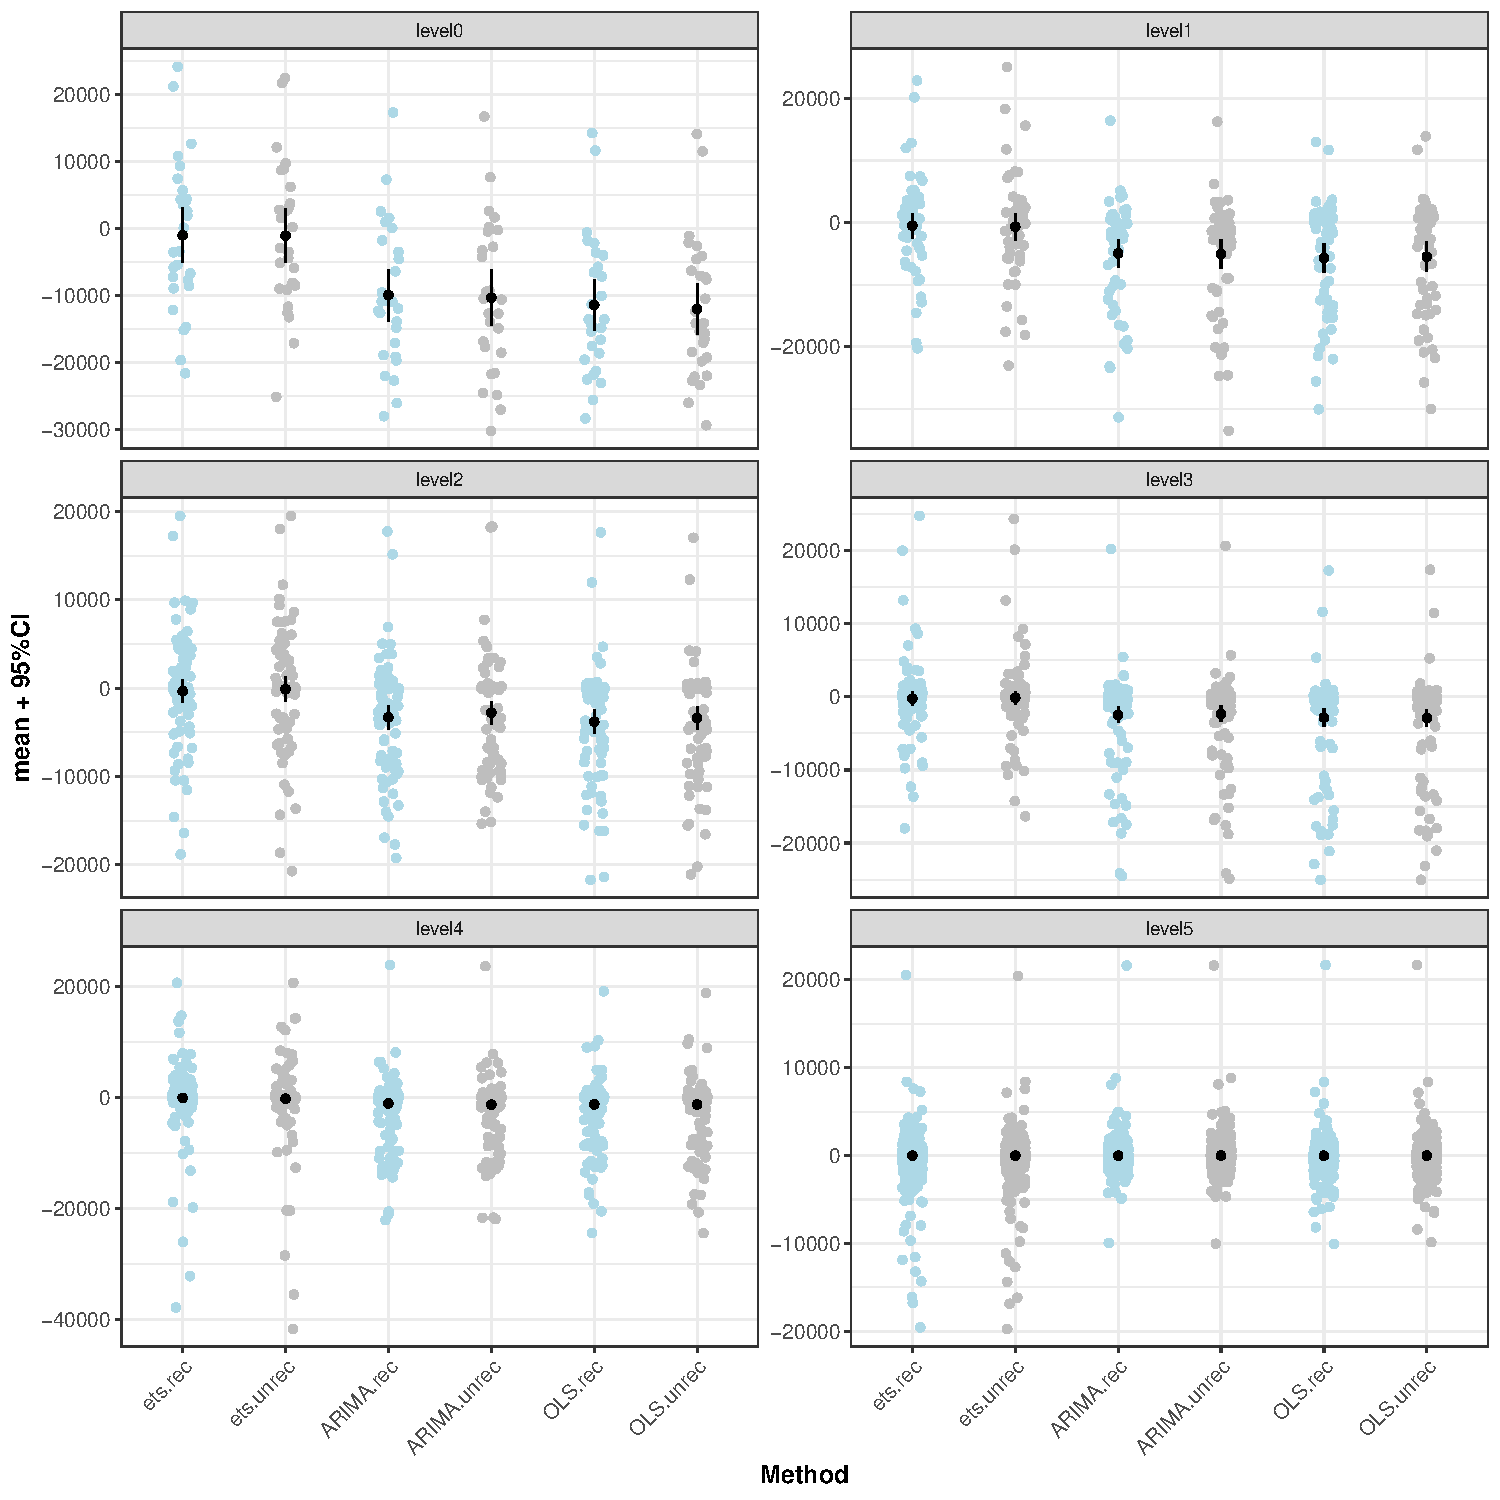
\includegraphics[width=400px,height=300px]{Paper-Figures/results_Wikipedia/boxplot_raw_data_1} 

}

\caption{Mean error plots with raw data -  Reconciled and unreconciled ets, ARIMA and OLS in all the hierarchy level- 1-step-ahead - Wikipedia dataset}\label{fig:errorplotrollingwiki}
\end{figure}

\begin{table}[t]

\caption{\label{tab:wikipediadataresultRMSE}Mean(RMSE) for ets, ARIMA and OLS with and without reconciliation - 28-step-ahead - Wikipedia dataset}
\centering
\begin{tabular}{ccccccc}
\toprule
\multicolumn{1}{c}{} & \multicolumn{6}{c}{Mean(RMSE)} \\
\cmidrule(l{2pt}r{2pt}){2-7}
\multicolumn{1}{c}{} & \multicolumn{3}{c}{Unreconciled} & \multicolumn{3}{c}{Reconciled} \\
\cmidrule(l{2pt}r{2pt}){2-4} \cmidrule(l{2pt}r{2pt}){5-7}
 & ets & ARIMA & OLS & ets & ARIMA & OLS\\
\midrule
Level 0 & 14846.93 & 24298.84 & 29840.58 & 14999.18 & 24649.91 & 29665.70\\
Level 1 & 13608.73 & 17277.01 & 21165.30 & 12240.30 & 16810.45 & 21048.06\\
Level 2 & 7117.43 & 10731.97 & 12678.89 & 7523.43 & 11068.81 & 12811.18\\
Level 3 & 6475.90 & 9580.38 & 12056.62 & 6509.03 & 9799.11 & 12112.46\\
Level 4 & 5302.74 & 8611.25 & 8451.09 & 5307.34 & 8239.77 & 8460.35\\
Level 5 & 435.64 & 390.05 & 389.41 & 437.67 & 391.22 & 390.97\\
\bottomrule
\end{tabular}
\end{table}

\begin{figure}

{\centering 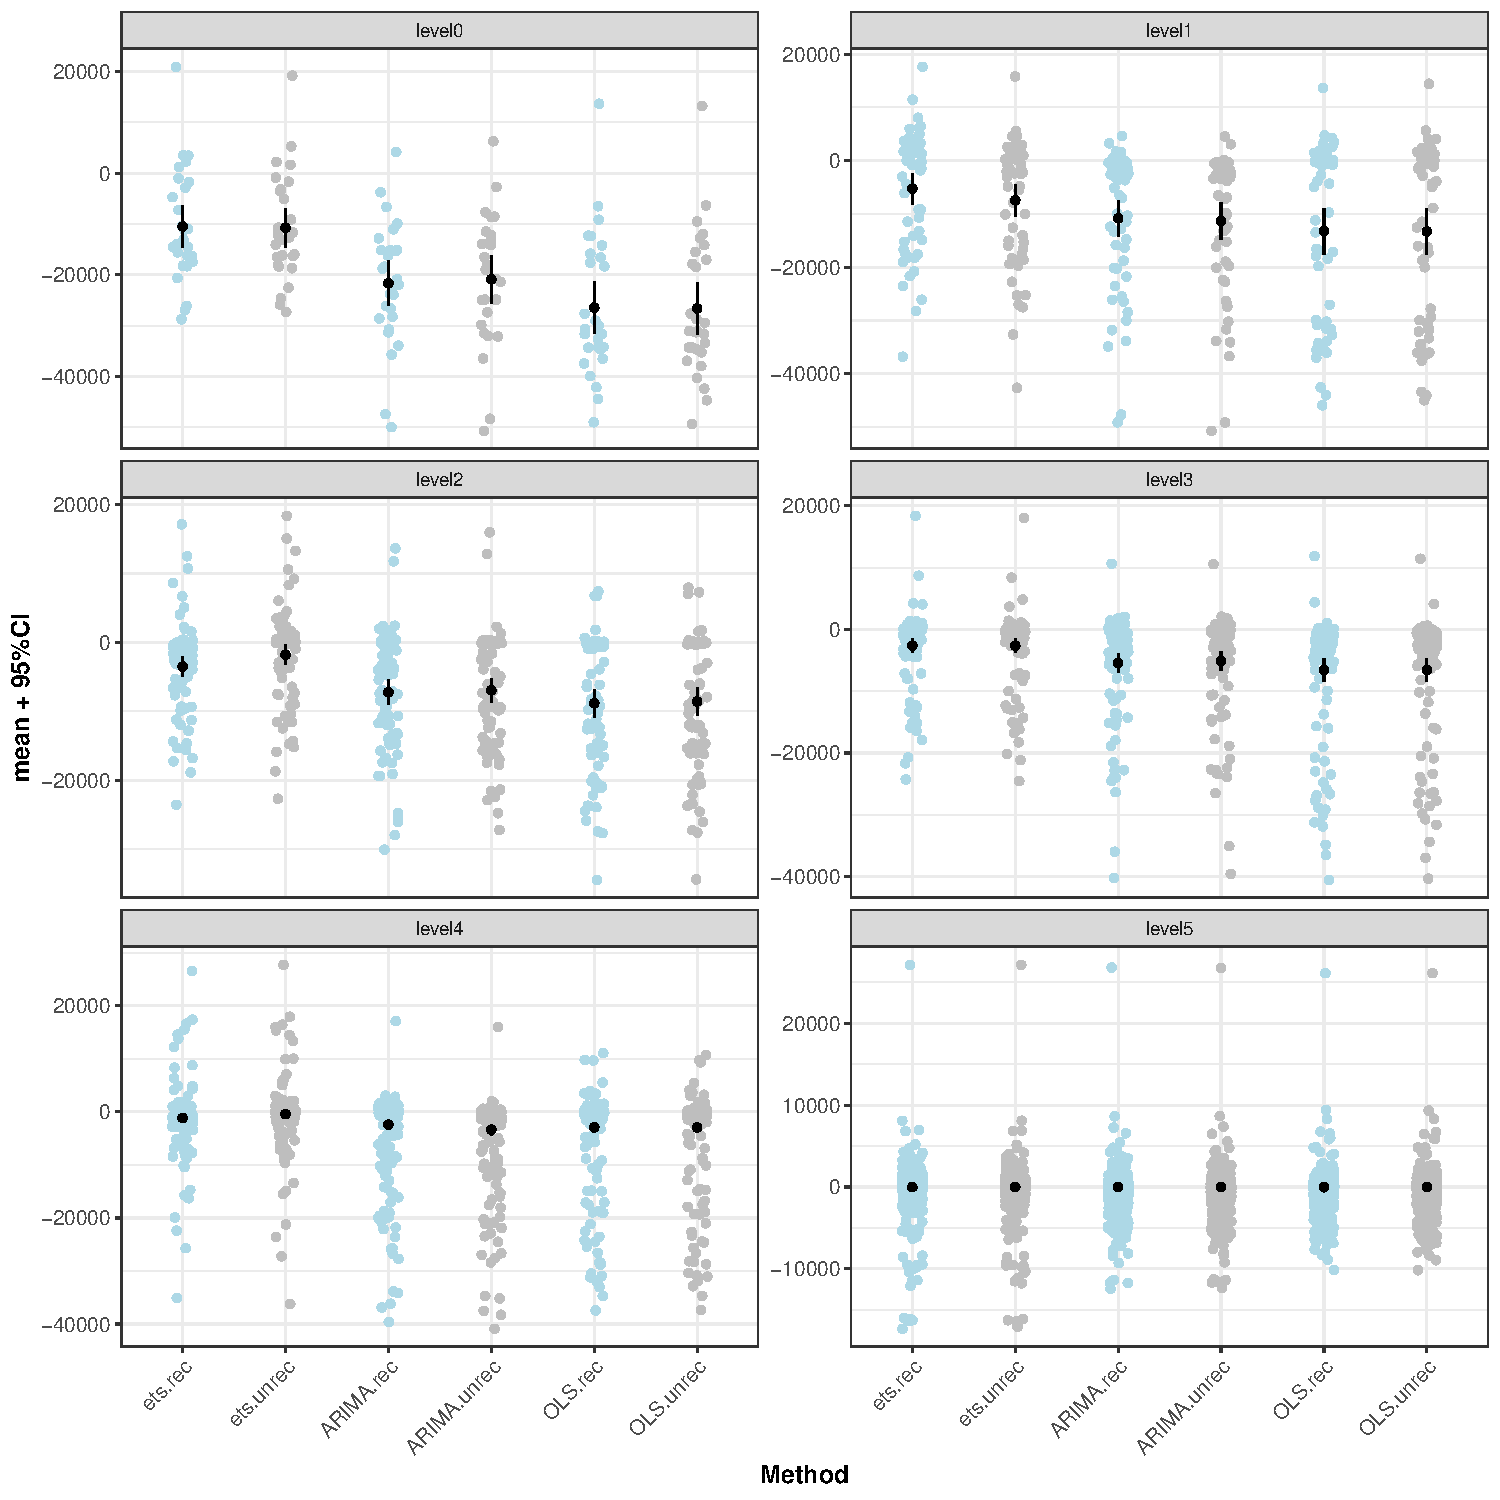
\includegraphics[width=400px,height=300px]{Paper-Figures/results_Wikipedia/boxplot_raw_data} 

}

\caption{Mean error plots with raw data -  Reconciled and unreconciled ets, ARIMA and OLS in all the hierarchy level- 28-step-ahead - Wikipedia dataset}\label{fig:errorplot28wiki}
\end{figure}

In Figure \ref{fig:forecstrolling24wiki}, we display a comparison among
one of the bottom level series, desktopusenPho
(desktop-user-english-photo sharing), actual test data and 1- and
28-step-ahead forecast results for ets, ARIMA and OLS, with (solid
lines) and without (dashed lines) applying reconciliation step. Based on
these plots, forecasting results based on our method is close to the
other two methods and reconciliation step can adjust our forecasts.

\begin{figure}

{\centering 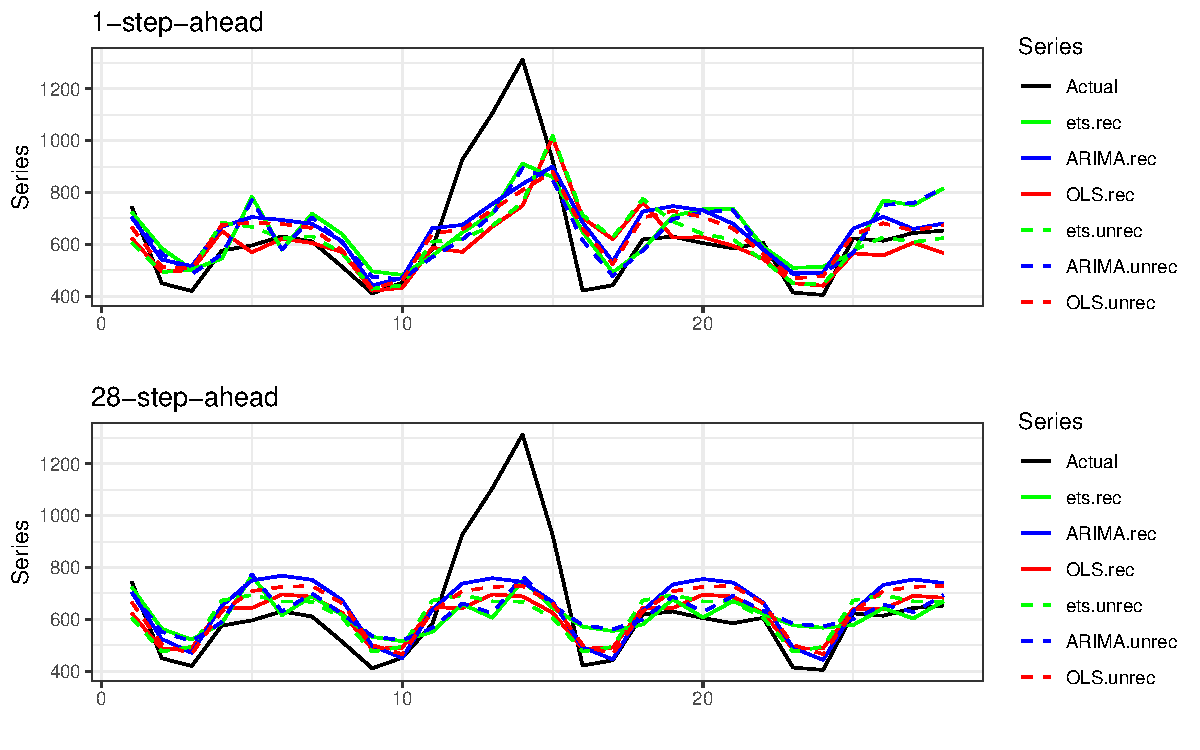
\includegraphics[width=400px,height=300px]{hcf_files/figure-latex/forecstrolling24wiki-1} 

}

\caption{Comparing Actual test set, Reconciled and unreconciled ets, ARIMA and OLS for desktopusenPho (desktop-user-english-photo sharing)  bottom level series- 1- and  28-step-ahead - Wikipedia dataset}\label{fig:forecstrolling24wiki}
\end{figure}

Lastly Table \ref{tab:wikipediadatacomputationtime} represent the
computation time for all three methods. You can see that ets and ARIMA
are much more computationally heavy in compare with OLS and running
reconciliation step cause not any tangible effect in computation time.

\begin{table}[t]

\caption{\label{tab:wikipediadatacomputationtime}Computation time (seconds) for ets, ARIMA and OLS with and without reconciliation - 1- and 28-step-ahead - Wikipedia dataset}
\centering
\begin{tabular}{>{\centering\arraybackslash}p{3cm}>{\centering\arraybackslash}p{3cm}>{\centering\arraybackslash}p{3cm}cc}
\toprule
\multicolumn{1}{c}{} & \multicolumn{4}{c}{Computation time (secs)} \\
\cmidrule(l{2pt}r{2pt}){2-5}
\multicolumn{1}{c}{} & \multicolumn{2}{c}{1-step-ahead} & \multicolumn{2}{c}{28-step-ahead} \\
\cmidrule(l{2pt}r{2pt}){2-3} \cmidrule(l{2pt}r{2pt}){4-5}
 & Unreconciled & Reconciled & Unreconciled & Reconciled\\
\midrule
ets & 13963.93 & 13963.96 & 450.89 & 450.92\\
ARIMA & 10327.02 & 10327.15 & 670.40 & 670.44\\
OLS & 82.55 & 82.62 & 35.39 & 35.43\\
\bottomrule
\end{tabular}
\end{table}

\section{Conclusion}\label{conclusion}

In this research we are proposing an approach to forecast hierarchical
time series faster. In the available package fore forecasting
hierarchical time series, \textbf{hts}, we can apply ets, ARIMA and RW
to to compute base forecast. Although ets and ARIMA are good in terms of
forecasting power and accuracy, they can be computationally heavy when
facing large collection of time series in hierarchy. Then adding another
faster option for calculating base forecasts was our purpose in this
research. Here we suggest a linear model, OLS, instead of ets and ARIMA
which is not computationally intensive. We also showed that OLS can
compete ets and ARIMA in terms of forecasting accuracy level. Another
good point of OLS is that it can handle missing data while ets and ARIMA
can not.

\section{Acknowledgements}\label{acknowledgements}

\printbibliography[title=References]

\end{document}
